
\subsection{Product perspective}

\begin{center}
White class are dedicated to perform Data4Help service, the other two applications are listed below.
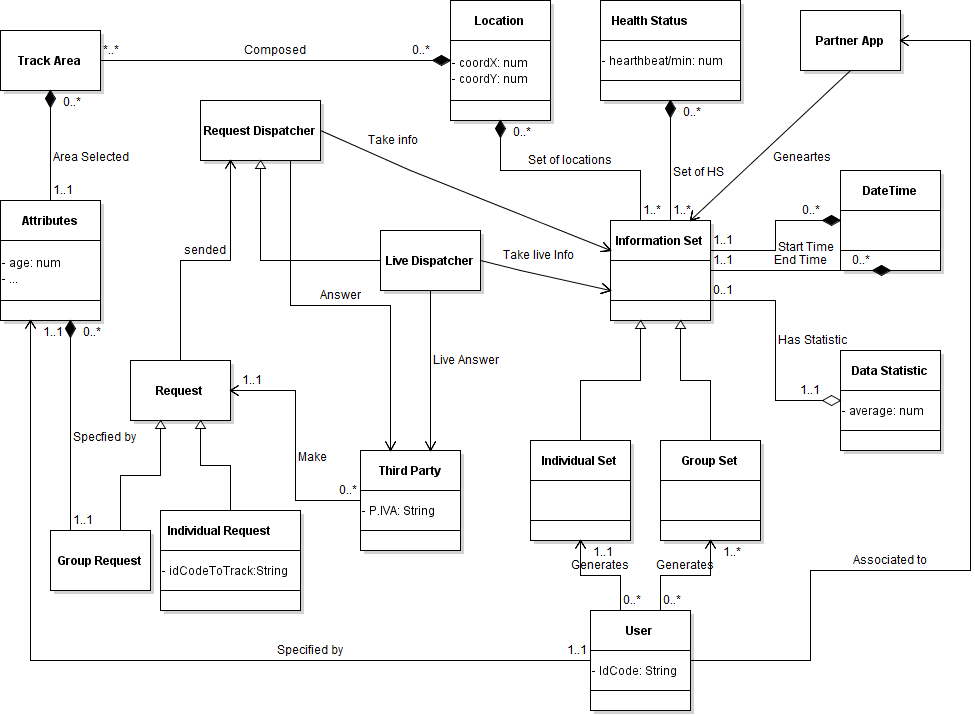
\includegraphics[scale=0.5]{Images/Class_Data4Help.png}
\end{center}

\begin{center}
{\color{Salmon} Red classes} are dedicated to {\color{Salmon} AutomatedSOS} application, supported by Data4Help service (White ones).
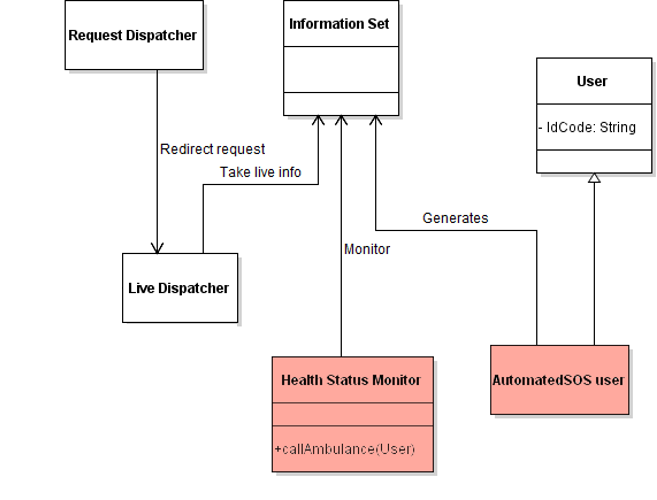
\includegraphics[scale=0.5]{Images/Class_AutoSOS.png}
\end{center}

\begin{center}
{\color{LimeGreen} Green classes} are dedicated to {\color{LimeGreen} Track4Run} application, supported by Data4Help service (White ones).
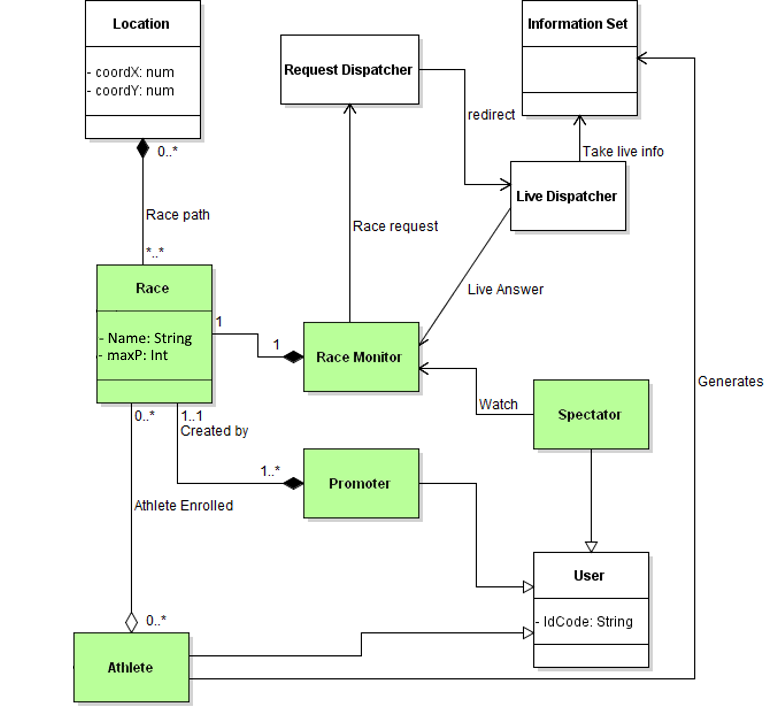
\includegraphics[scale=0.5]{Images/Class_Track4Run.png}
\end{center}


\subsection{Product functions}
Here we include the most important requirements in word

\subsection{User characteristics}
\begin{enumerate}
\item Third Party: Registered company interested in retrieve useful data from TrackMe's users. Usually this information can be useful for marketing strategy.
	\begin{enumerate}
		\item Health Third Party: Non-Profit Company interested to monitor 		individuals in order to prevent critical diseases. 
	\end{enumerate}
\item User: Individual that provides information about himself. His privacy must be protected by the system.
	\begin{enumerate}
		\item Athlete: Track4Run's user that is enrolled in one or more race.
		\item Promoter: Track4Run's user that is the promoter of one or more race.
		\item Spectator:Track4Run's user that want follow athletes in one or more race.
	\end{enumerate}
\end{enumerate}

\subsection{Assumptions, dependencies and constraints}
In the specification document certain parts were not specific and were ambiguous. So we decided to make the following assumptions.

\subsubsection{Text Assumptions}
\begin{enumerate}

\item[•] {\Large Data4Help}
	\begin{enumerate}
	\item Users' information are collected from partner applications on users' devices.
	\item For example all the fitness application developed for smartwatch can be partner applications, also AutomatedSOS and Track4Run can be them as well.
	\item Only registered third parties can request monitoring service.
	\item Groups are characterized by its member’s attributes (age, gender, city, etc…).
	\item Discriminative attributes are all the credentials inserted by user (i.e. age, job etc...), their location more or less precise (country, region, city, neighbourhood ..) and the period of time interested (days, weeks, months..).
	\item Third parties in group mode are interested in number of users that match attribute specified, their location statistics and the statistics of group health status.
	\item Group mode acquisition can be performed without user's agreement.
	\item Third parties in single mode are interested to retrieve the sequence of position and health status information, detected from a certain users during a selected time period.	
	\item Single mode acquisition cannot be performed without user's agreement.
	\item Health status parameters acquirable are all the ones supported by a standard smartwatch as: Heart Rate, Blood Pressure, Pedometer, Calories Calculation.
	\item Geographic location can be retrieved either by smartwatch or smartphone.
	\end{enumerate}
	
\item[•] {\Large AutomatedSOS}
	\begin{enumerate}
	\item For this service individuals subscribe to a single Third Party and not the other way around.
    \item Third parties interested in this type of service are only non-profit organizations that want to rescue individuals in a faster way.
    \item Different third parties cannot receive information from the same user (Otherwise both send the same SOS request).
    \item This service can be used only by elderly people (70+) or by who really need it, to avoid useless waste of resources. 
	\end{enumerate}
	
\item[•] {\Large Track4Run}
	\begin{enumerate}
	\item Any user can organize an event.
    \item An event can be public or private.
    \item If the event is private then, the organizer need to know the security number or the fiscal code of the athletes to invite.
    \item If the event is public then the only restriction is in the number of athletes admitted.
    \item All the events can be followed by everyone as spectator.
    \item All users invited to an event can accept or discard the request.
    \item Race path are always composed by citizen routes (never in private circuits or stadiums)
    \end{enumerate}
\end{enumerate}

\subsubsection{Domain Assumptions}
\begin{enumerate}

\item[•] {\Large Data4Help}
	\begin{enumerate}
	\item [D.1.1] Users' information collected are coming from installed app on users' smartphone/smartwatch, that are partner of TrackMe.
	\item [D.1.2] Whenever an individual download a partner application and through registration accepts its policy, he agrees to TrackMe's policy too.
	\item [D.1.3] The identification (fiscal code, social security number) and the secondary data (attributes) given by the individual during the registration are correct.
    \item [D.1.4] Individuals must always dress a smartwatch that retrieve health parameters and user's positions.
    \item [D.1.5] Devices used to monitor individuals always work and report the correct values.
    \item [D.1.6]
	\item [D.1.7] In order to perform single mode acquisition, third parties has to insert fiscal code of tracked user (aka: nor security number neither fiscal code are visible on the application).
	\item [D.1.8] In order to perform group mode acquisition, third parties have to select attributes of individuals in which they are inserted.
	\end{enumerate}
	
\item[•] {\Large AutomatedSOS}
	\begin{enumerate}
	\item [D.2.1] All devices used to monitor the health of the individual always work and report the correct values.
    \item [D.2.2] The ambulance successfully reach the location of the individual.
    \item [D.2.3] The ambulance always get to the location in the minimum amount of time.
    \item [D.2.4] As soon as the parameters get below the threshold, the ambulance gets notified
    \item [D.2.5] Third parties that want to exploit this service need to enable the individual registration function.
    \item [D.2.6] Users' interested must equip with smartwatch that supports health status acquisition and install AutomatedSOS application on it.
	\end{enumerate}
	
\item[•] {\Large Track4Run}
	\begin{enumerate}
	\item [D.3.1] The path defined by the organizer actually exist
    \item [D.3.2] If an athlete enroll to a run then he also participates to the run.
    \item [D.3.3] All athletes have their tracking devices with them for the entire duration of the run.
    \item [D.3.4] Athletes never go out of the defined path defined.
    \item [D.3.5] Users' interested must equip with smartphone that supports location acquisition and install Track4Run application on it.
	\end{enumerate}
	
\end{enumerate}